\begin{figure}
\begin{fullpage}

\begin{center}
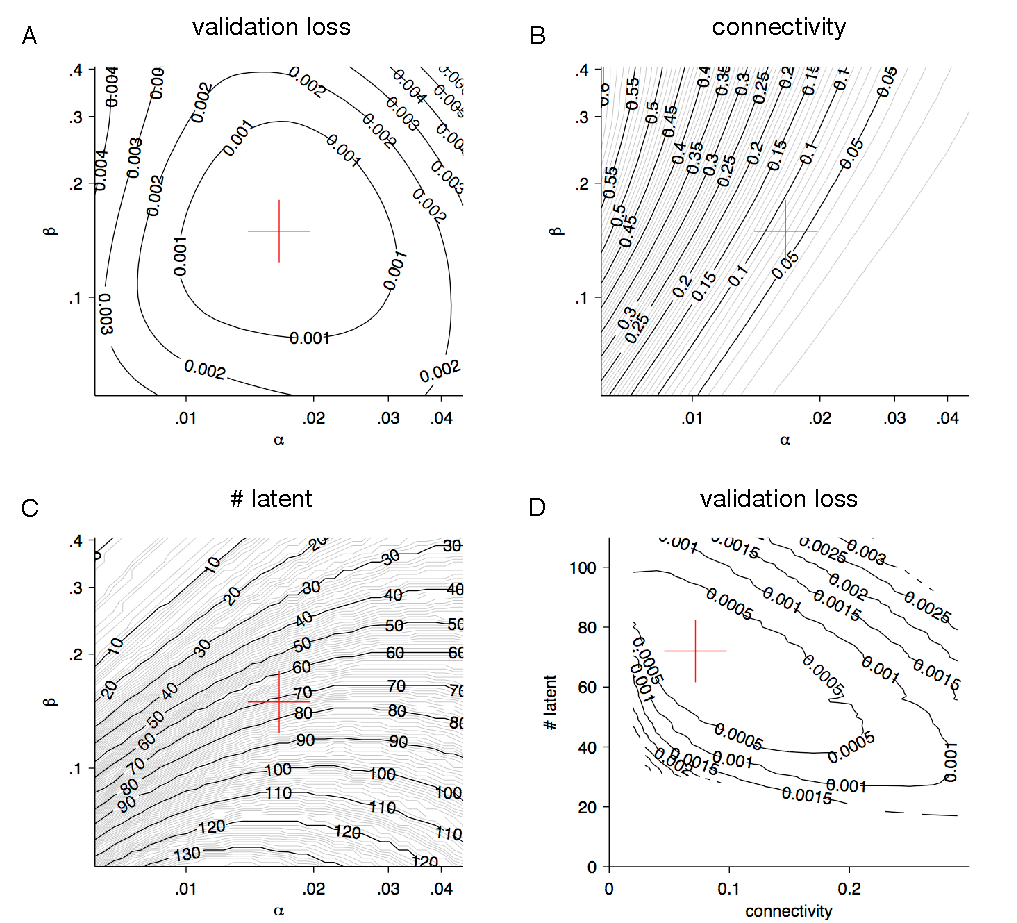
\includegraphics[width=\textwidth]{./figures/Supp1.pdf}
\end{center}

\caption[Optimization of regularization parameters]{
{\bf Optimization of regularization parameters of the $C_{\sf sparse+latent}$ estimator.} {\bf A.} Validation loss (Eq.~\ref{eq:full-loss}) for the example site in Fig.~\ref{fig:2} and \ref{fig:4} as a function of the hyperparameters $\alpha$ and $\beta$ of the $C_{\sf sparse+latent}$ estimator (Eq.~\ref{eq:c-sl} and Eq.~\ref{eq:ma}). In all panels, the red cross marks the optimal value found by the pattern search algorithm described in Methods.
{\bf B.} The connectivity ($1-\mbox{sparsity}$) of the sparse component $S$ as a function of $\alpha$ and $\beta$ for the example site.
{\bf C.} The number of latent units, \emph{i.e.}~the rank of the low-rank component $L$, as a function of hyperparameters $\alpha$ and $\beta$.
{\bf D.} The loss function as a function of the connectivity and the number of latent units.
}\label{fig:S1}
\end{fullpage}
\end{figure}